\documentclass[conference,a4paper]{IEEEtran}
\IEEEoverridecommandlockouts
% The preceding line is only needed to identify funding in the first footnote. If that is unneeded, please comment it out.
%Template version as of 6/27/2024

\usepackage{url}
\usepackage{cite}
\usepackage{amsmath,amssymb,amsfonts}
\usepackage{algorithmic}
\usepackage{graphicx}
\usepackage{textcomp}
\usepackage{xcolor}
\usepackage{tabularx}
\usepackage{booktabs}
\usepackage{multirow}
\usepackage{enumitem}

\def\BibTeX{{\rm B\kern-.05em{\sc i\kern-.025em b}\kern-.08em
    T\kern-.1667em\lower.7ex\hbox{E}\kern-.125emX}}
\begin{document}

\title{Hungarian Pseudo-Hierarchies for Coarse-to-Fine Ultra Fine-Grained Image Recognition}

\author{Anonymous Authors}

\maketitle

\begin{abstract}
Ultra-fine-grained image recognition (UFGIR) is the task of distinguishing sub-categories within a species, such as different cultivars of a plant, extending beyond traditional fine-grained recognition of visually similar species. Hierarchical supervision has been shown to improve FGIR performance by introducing structured relationships among classes, but constructing such hierarchies requires costly human annotation, limiting its applicability in specialized domains where taxonomies are unavailable. To address this limitation, we propose Hungarian Pseudo-Hierarchy (HPH), a method that automatically generates hierarchical structures from fine-grained labels without human annotation and leverages curriculum learning to improve fine-grained recognition. We evaluate HPH across 21 pretrained convolutional and transformer backbones on the ultra fine-grained SoyLocal dataset, and further validate its effectiveness on the Cotton and SoyAgeing-R1 datasets. HPH consistently improves classification accuracy over non-hierarchical baselines, achieving absolute gains of up to \textbf{22.3\%} across backbone. Furthermore, HPH consistently improves performance, achieving improvements of up to \textbf{18.16\%} on datasets containing only \textbf{3--5 training images per class} from previous state-of-the-art (SoTA) method, demonstrating that automatically generated pseudo-hierarchies provide an effective and scalable alternative to manually annotated taxonomies for fine-grained image recognition.
\end{abstract}

\begin{IEEEkeywords}
Hierarchical, Multi-label classification, Computer vision, Multi-taxonomy learning, Pseudo-hierarchy.
\end{IEEEkeywords}

\section{Introduction}
Fine-grained image recognition (FGIR) aims to distinguish between visually similar subcategories within a broader class. Ultra-fine-grained image recognition (UFGIR) pushes this granularity even further, targeting categories such as plant cultivars, where visual differences are so subtle that even domain experts often struggle to distinguish them \cite{yu_benchmark_2021}. Many FGIR problems can naturally be organized into taxonomic hierarchies (e.g., family, genus, species), allowing hierarchical FGIR methods to exploit coarse-level supervision to improve fine-grained recognition compared with treating labels as flat categories \cite{zhang_part-based_2014, zheng_learning_2017, chen_fine-grained_2018, chang_your_2021}. However, such taxonomies rarely exist for the cultivar-level categories targeted by UFGIR, making hierarchical supervision difficult to apply in practice.

The absence of hierarchical structure prevents existing hierarchical FGIR methods from being directly applied to UFGIR. Constructing a taxonomy manually requires substantial domain expertise and is often impractical for specialized datasets. This raises a fundamental question: can an automatically constructed pseudo-hierarchy provide the benefits of hierarchical supervision for UFGIR?

In this work, we propose Hungarian Pseudo-Hierarchy (HPH), a method that automatically constructs pseudo-hierarchies from fine-grained labels. HPH forms super-categories by grouping semantically related fine-grained classes using bipartite matching, producing a multi-level label hierarchy for supervision during training. This structure naturally leverages curriculum learning \cite{bengio_curriculum_2009}, where backbones first learn easier coarse-level classification before progressing to more challenging fine-grained classification. As a result, existing hierarchical FGIR frameworks can be readily applied to UFGIR datasets, where curriculum learning progressively guides optimization from coarse categories to fine-grained classes, improving performance even in challenging and low-resource UFGIR datasets.

Our study offers three main contributions:
\begin{enumerate} [topsep=3pt, itemsep=2pt, parsep=1pt]
    \item We propose \textbf{Hungarian Pseudo-Hierarchy (HPH)}, a pseudo-hierarchy construction method that alleviates the absence of hierarchical supervision in UFGIR by automatically generating hierarchical labels from fine-grained classes through Hungarian bipartite matching.
    \item We conduct a large-scale empirical study on fine-grained image recognition using 21 pretrained backbones (11 CNNs and 10 ViTs) on SoyLocal dataset, and further validate our findings on the Cotton and SoyAgeing-R1 datasets using 2 backbones, ViT and DeiT.
    
    \item HPH consistently improves classification accuracy across diverse backbone architectures and low-resource UFGIR datasets, achieving gains of up to \textbf{22.3\%} over non-hierarchical baselines and up to \textbf{18.16\%} on datasets containing only \textbf{3--5 training images per class} from previous SoTA method.

\end{enumerate}

\begin{figure*}[!htb]
    \centering
    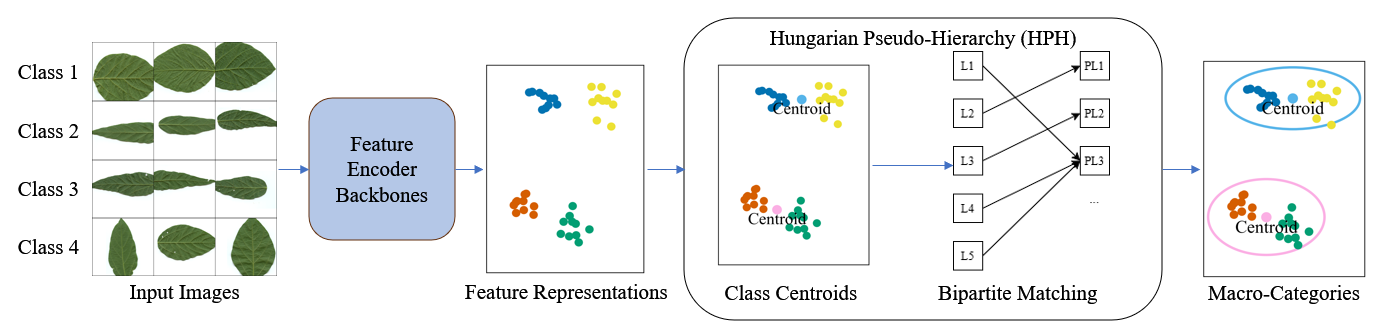
\includegraphics[width=1\textwidth]{figures/overview.png}
    \caption{Overview of the Hungarian Pseudo-Hierarchy (HPH) construction. Input images are encoded into feature representations, from which class centroids are computed for each fine-grained category $L_i$. A bipartite matching formulation using the Hungarian algorithm groups these classes into pseudo coarse categories $PL_j$, forming a two-level pseudo-hierarchy for hierarchical supervision.}
    \label{fig_overview}
\end{figure*}

\section{Related Works}
\label{sec_related}
\subsection{Hierarchical Consistency Learning}
A key line of work in Hierarchical Fine-Grained Image Recognition (HFGIR) focuses on enforcing consistency between predictions at different semantic levels through architectural designs or loss functions. Early methods such as HSE \cite{chen_fine-grained_2018} adopt coarse-to-fine sequential prediction with hierarchical regularization, while later approaches including HRN \cite{chen_label_2022} and SAHC \cite{weikmann_semantics-aware_2025} improve consistency using feature fusion or divergence-based objectives. Lozachmeur et al. \cite{lozachmeur_hierarchical_2025} proposed a modular multi-label hierarchical learning framework for industrial image recognition that incorporates hierarchy-aware prediction head. These methods impose hierarchical constraints within the training objective or model architecture to ensure agreement across label levels. In contrast, our method constructs pseudo-hierarchies as an external preprocessing step, making it directly compatible with existing hierarchical learning frameworks.

\subsection{Pseudo-Hierarchies in Image Classification}
Pseudo-hierarchies aim to recover hierarchical structure from data when ground-truth taxonomies are unavailable. Existing approaches typically construct hierarchies by clustering embeddings or logits, often in a top-down manner to induce semantic groupings \cite{zheng_online_2021, palumbo_logits_2025}. Other methods explore hierarchical organization through probabilistic or prototype-based representations \cite{wang_deep_2025, hsieh_pseudo-label_2019}. In contrast, our method constructs pseudo-hierarchies in a bottom-up manner by merging fine-grained classes into coarser groups using pretrained feature representations and existing labels, facilitating hierarchical supervision under fine-grained settings.

\section{Learning with Hungarian Pseudo-Hierarchy}
\label{sec_method}
Our approach consists of three stages: 1. Feature extraction, 2. Pseudo-hierarchy construction, and 3. Hierarchical training, as illustrated in Fig. \ref{fig_overview}.

\subsection{Feature Representation Extraction}
Features are extracted from backbones. For Resnet models, we use the last second BatchNorm layer  of the final block, while for ViT-based models we use last second LayerNorm of the encoder. Adaptive average pooling is applied when necessary to obtain a fixed-dimensional representation.

Given an input image $x$, the feature extractor $\phi(\cdot)$ produces
\[
\mathbf{z} = \phi(x) \in \mathbb{R}^{D}.
\]
Aggregating features from all training samples yields the feature set $Z \in \mathbb{R}^{M \times D}$, where $M$ is the number of training samples and $D$ is the feature dimension.

\subsection{Pseudo-Hierarchy Construction}
To alleviate the cost of manually annotating hierarchical labels, we propose \textbf{Hungarian Pseudo-Hierarchy (HPH)}, which constructs hierarchical structures from fine-grained class features. HPH groups semantically similar classes into pseudo-coarse categories based on centroid representations, forming a multi-level structure that can be used for supervision. This process naturally induces a curriculum learning strategy by organizing training from coarse to fine granularity.

Given the extracted feature representations, each fine-grained class is represented by its centroid
\[
\mathbf{m}_i
=
\frac{1}{|\mathcal{S}_i|}
\sum_{x\in\mathcal{S}_i}
\phi(x),
\]
where $\mathcal{S}_i$ denotes the set of training samples belonging to fine-grained class $i$, and $\mathbf{m}_i\in\mathbb{R}^{D}$ is the corresponding class centroid.


The pairwise Euclidean distances between class centroids are then computed to form the distance matrix
\[
A_{ij}
=
\left\|
\mathbf{m}_i-\mathbf{m}_j
\right\|_2,
\qquad
A\in\mathbb{R}^{K\times K},
\]
where $K$ is the number of fine-grained classes.

Since the desired number of pseudo-coarse classes $L$ is smaller than $K$, the distance matrix is padded before applying the Hungarian algorithm \cite{kuhn_hungarian_1955}. Fine-grained classes assigned to padded columns are subsequently reassigned to the nearest valid pseudo-coarse class based on centroid distance, producing a two-level pseudo-hierarchy.

\subsection{Hierarchical Classification Module}
Given a hierarchy constructed either from manual annotation or the proposed pseudo-hierarchy generation process, prediction is performed using a hierarchical multi-granularity classification framework following Chang et al. \cite{chang_your_2021}. In this setting, each image is associated with labels ordered from coarse to fine granularity. The objective is a multi-task learning problem in which classifiers at different semantic levels are learned jointly.

Let the backbone network produce a feature representation $\mathbf{z}$ for an input image $x$. For a hierarchy with $K$ levels, the shared feature is forwarded to $K$ classification heads ${g_k(\cdot)}_{k=1}^{K}$, where each head predicts a probability distribution over the label space of its corresponding level with the formula below:
\[
\mathbf{p}^{(k)} = g_k(\mathbf{z}), \quad k = 1, \dots, K,
\]

Training is performed using $\mathcal{L}_{\text{CE}}$ computed independently at every hierarchy level. The overall hierarchical loss is the sum of per-level losses:
\[
\mathcal{L} = \sum_{k=1}^{K} \mathcal{L}_{\mathrm{CE}}^{(k)}
\]
Each classifier therefore contributes to the overall optimization while sharing the same backbone representation. Each head supervises a different semantic level, while inference uses only the finest-level prediction.

\section{Experiment Setup}
\label{sec_setup}

We evaluate our approach on three Ultra Fine-Grained Image Recognition (UFGIR) datasets: SoyLocal, Cotton, and SoyAgeing-R1 \cite{yu_benchmark_2021}. We conduct a comprehensive study across 21 pretrained backbones for Soylocal. Then, the experiments extend to Cotton and SoyAgeing-R1 using 2 representative backbones, DeiT and ViT, to evaluate the effectiveness of HPH under low-resource.

Our experiments consider 21 backbones spanning two types, 10 Transformer (ViT-B) and 11 CNN (ResNet50). The ViT-B models include ViT~\cite{dosovitskiy_image_2020}, DeiT~\cite{touvron_deit_2022}, DeiT3-IN1K~\cite{touvron_deit_2022}, DeiT3-IN21K~\cite{touvron_deit_2022}, ViT-MIIL~\cite{ridnik_imagenet-21k_2021}, MoCoV3~\cite{chen_empirical_2021}, DINO~\cite{caron_emerging_2021}, SigLIP-v2~\cite{tschannen_siglip_2025}, CLIP-LAION5B~\cite{cherti_reproducible_2023}, and MAE~\cite{he_masked_2021}.  The ResNet50 models include Torchv1~\cite{he_deep_2016}, Torchv2~\cite{he_deep_2016}, Gluon~\cite{he_bag_2018}, A1~\cite{wightman_resnet_2021}, MIIL~\cite{ridnik_imagenet-21k_2021}, IG1B~\cite{yalniz_billion-scale_2019}, YFCC100M~\cite{yalniz_billion-scale_2019}, MoCoV3~\cite{chen_empirical_2021}, SupCon~\cite{khosla_supervised_2021}, SwAV~\cite{caron_unsupervised_2021}, and SparK~\cite{tian_designing_2023}.

To assess model effectiveness in hierarchical FGIR, we report the Top-1 classification accuracy at the finest level of the hierarchy (L1). While the hierarchical structure contains up to two levels (L2, and L1, from coarsest to finest), the coarse labels in the pseudo-hierarchy are automatically generated and do not correspond to ground-truth semantic labels. Therefore, the coarse-level accuracies are not meaningful for evaluation. As a result, we focus our analysis on the finest-level accuracy, which reflects the true classification performance on the original dataset labels.

We fine-tune all models for \textbf{200 epochs} on the SoyLocal dataset and \textbf{50 epochs} on the Cotton and SoyAgeing-R1 datasets using a batch size of 8. To study the impact of hyperparameters, we use two optimizers (SGD and AdamW) across 10 learning rates, SGD (0.3–0.003) with weight decay 0, and AdamW (0.005–0.000005) with weight decay 0.05. We employ cosine learning rate scheduler and mixed precision. During training, we employ standard data augmentation (resize to 550×550, random crop to 448×448, horizontal flip). Center cropping is used during inference.

We control the granularity of coarse-level pseudo-hierarchies using a \textbf{cluster ratio}, defined as the number of coarse labels relative to the number of fine-grained labels. For the SoyLocal dataset, we construct 2-level pseudo-hierarchies using seven cluster ratios: 10\%, 20\%, 30\%, 40\%, 50\%, 70\%, and 90\%. Based on the SoyLocal results, we evaluate only the two best-performing cluster ratios, 70\% and 90\%, on the Cotton and SoyAgeing-R1 datasets. These experiments evaluate how the granularity of pseudo-hierarchies affects hierarchical FGIR performance.


\begin{figure}[ht]
    \centering
    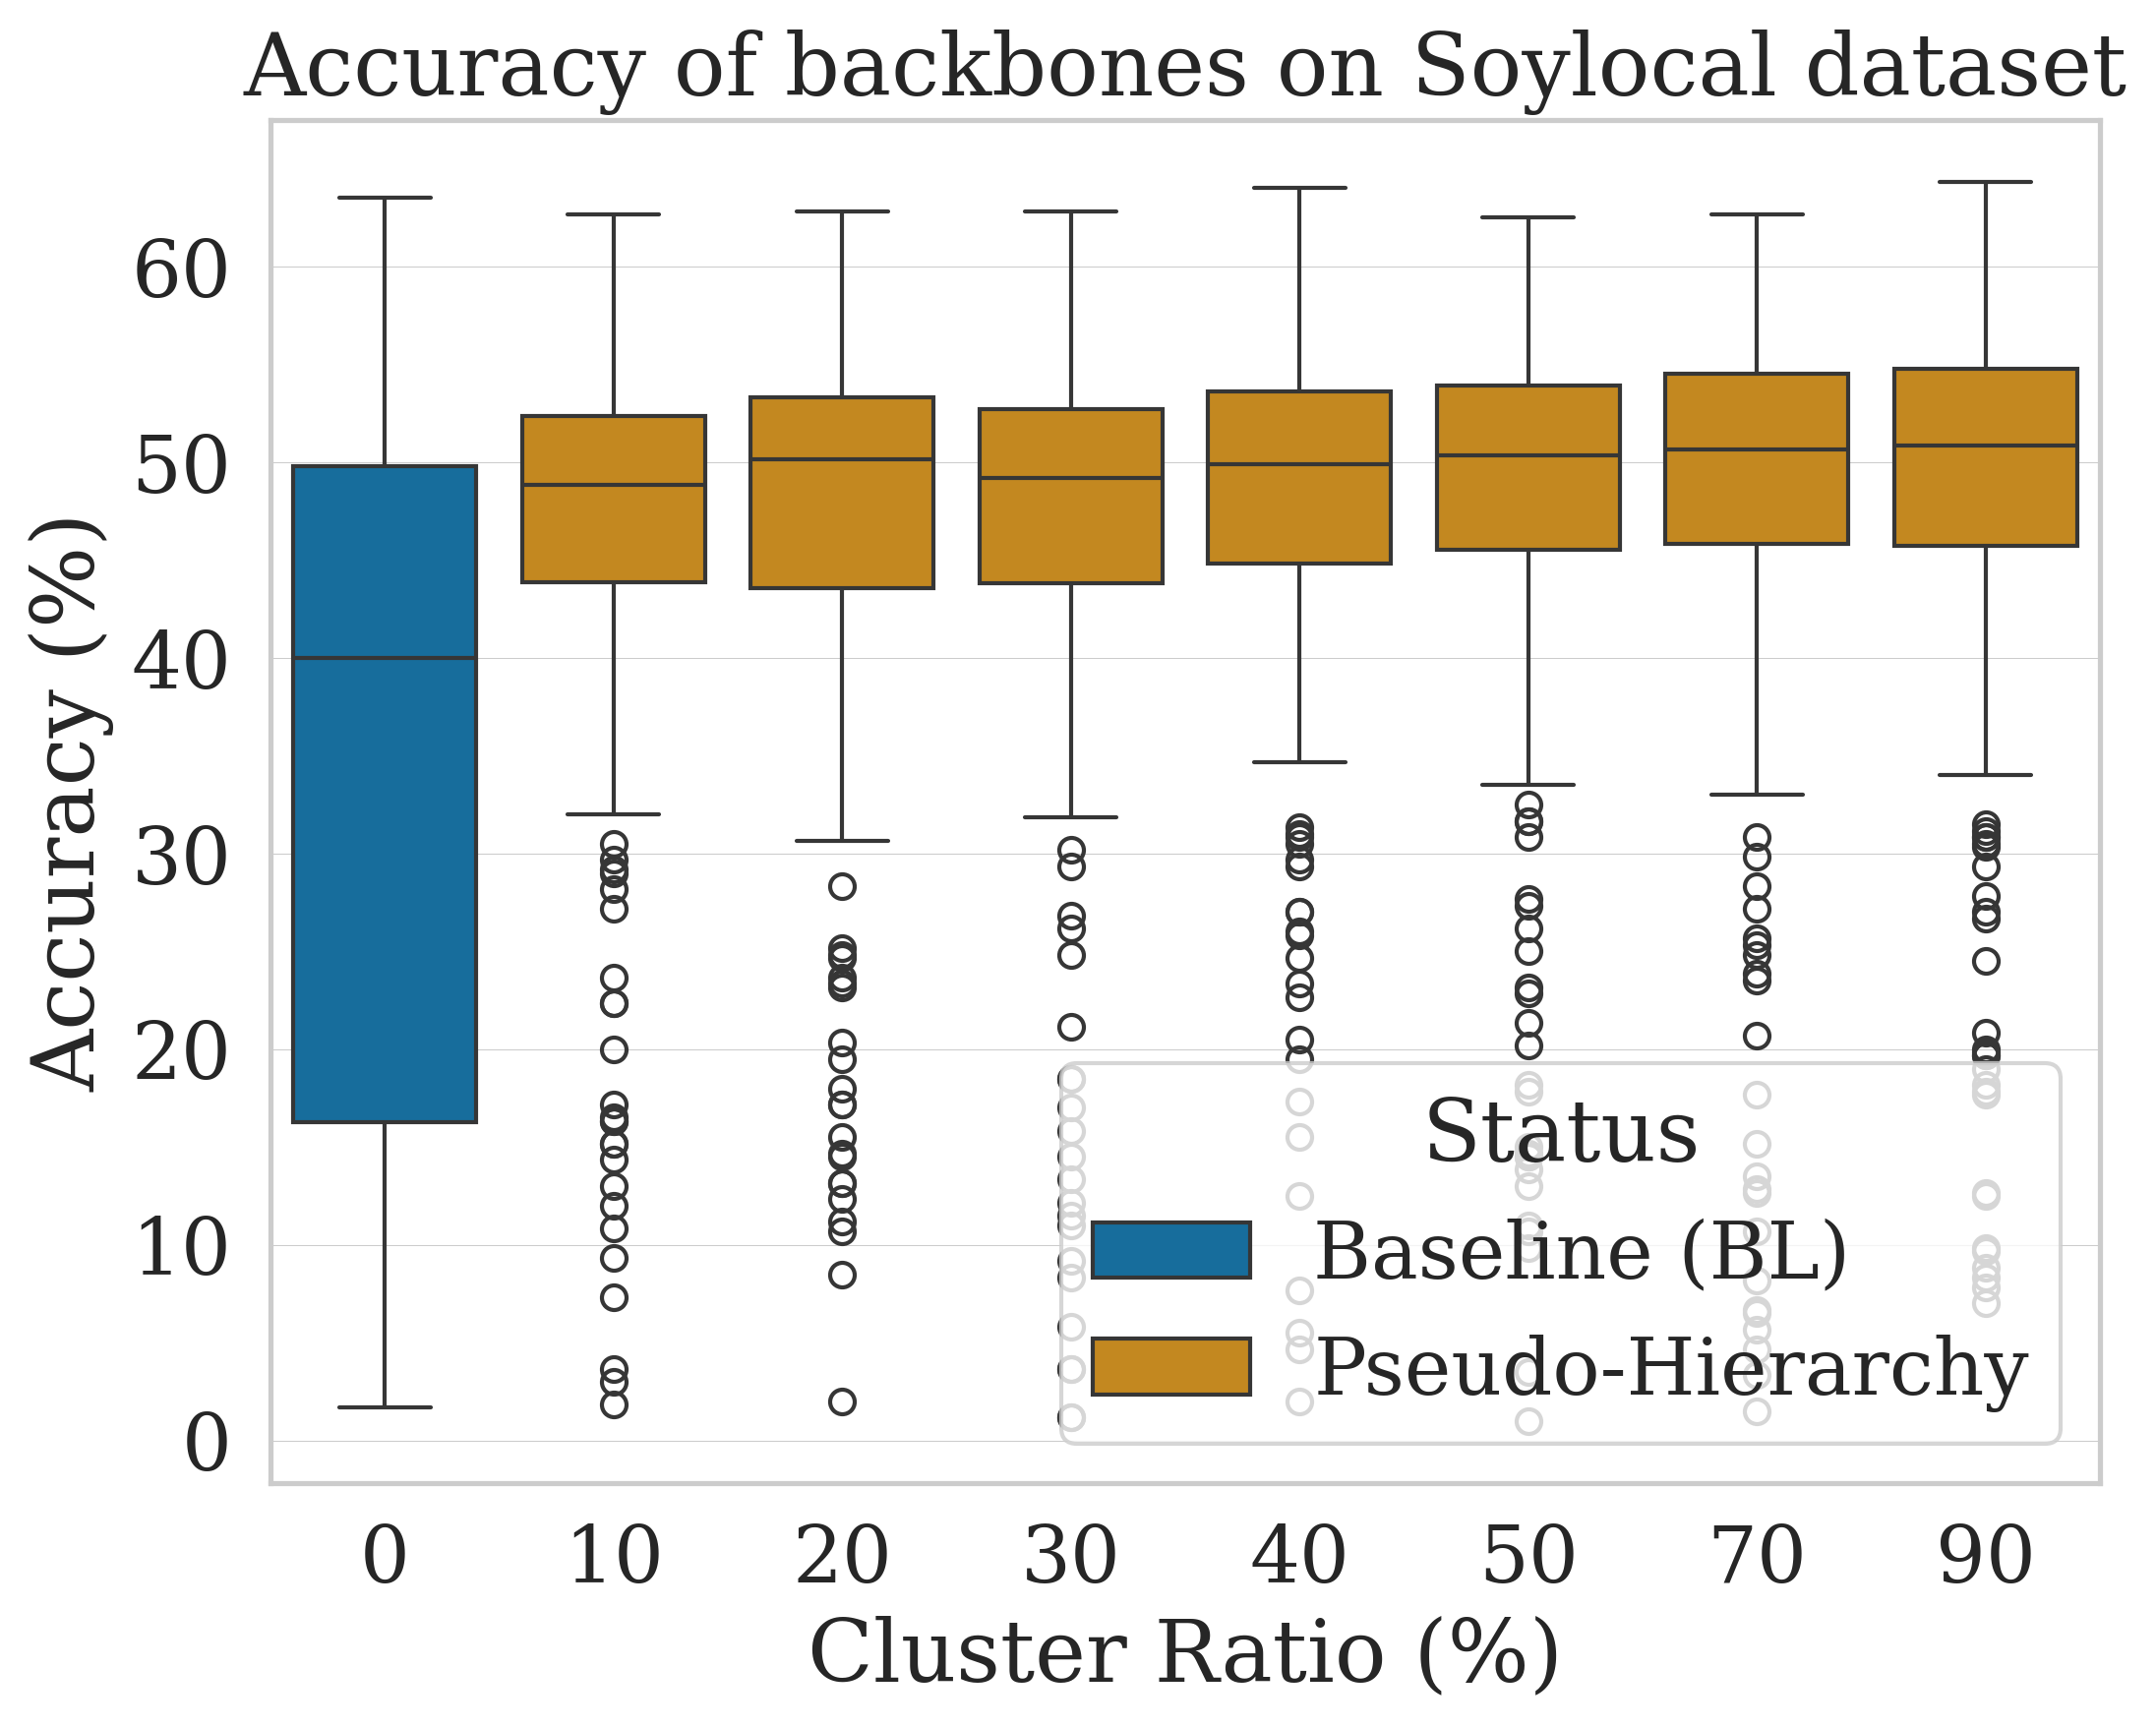
\includegraphics[width=0.75\linewidth]{figures/compare_soylocal.png}
    \caption{Comparison of 21 backbones on Soylocal dataset. 0\% Cluster Ratio represents baseline with no hierarchy, while others with HPH pseudo-hierarchy.}
    \label{fig_pseudo_soylocal}
\end{figure}

\begin{figure*}[!htb]
    \centering
    \begin{minipage}{0.48\linewidth}
        \centering
        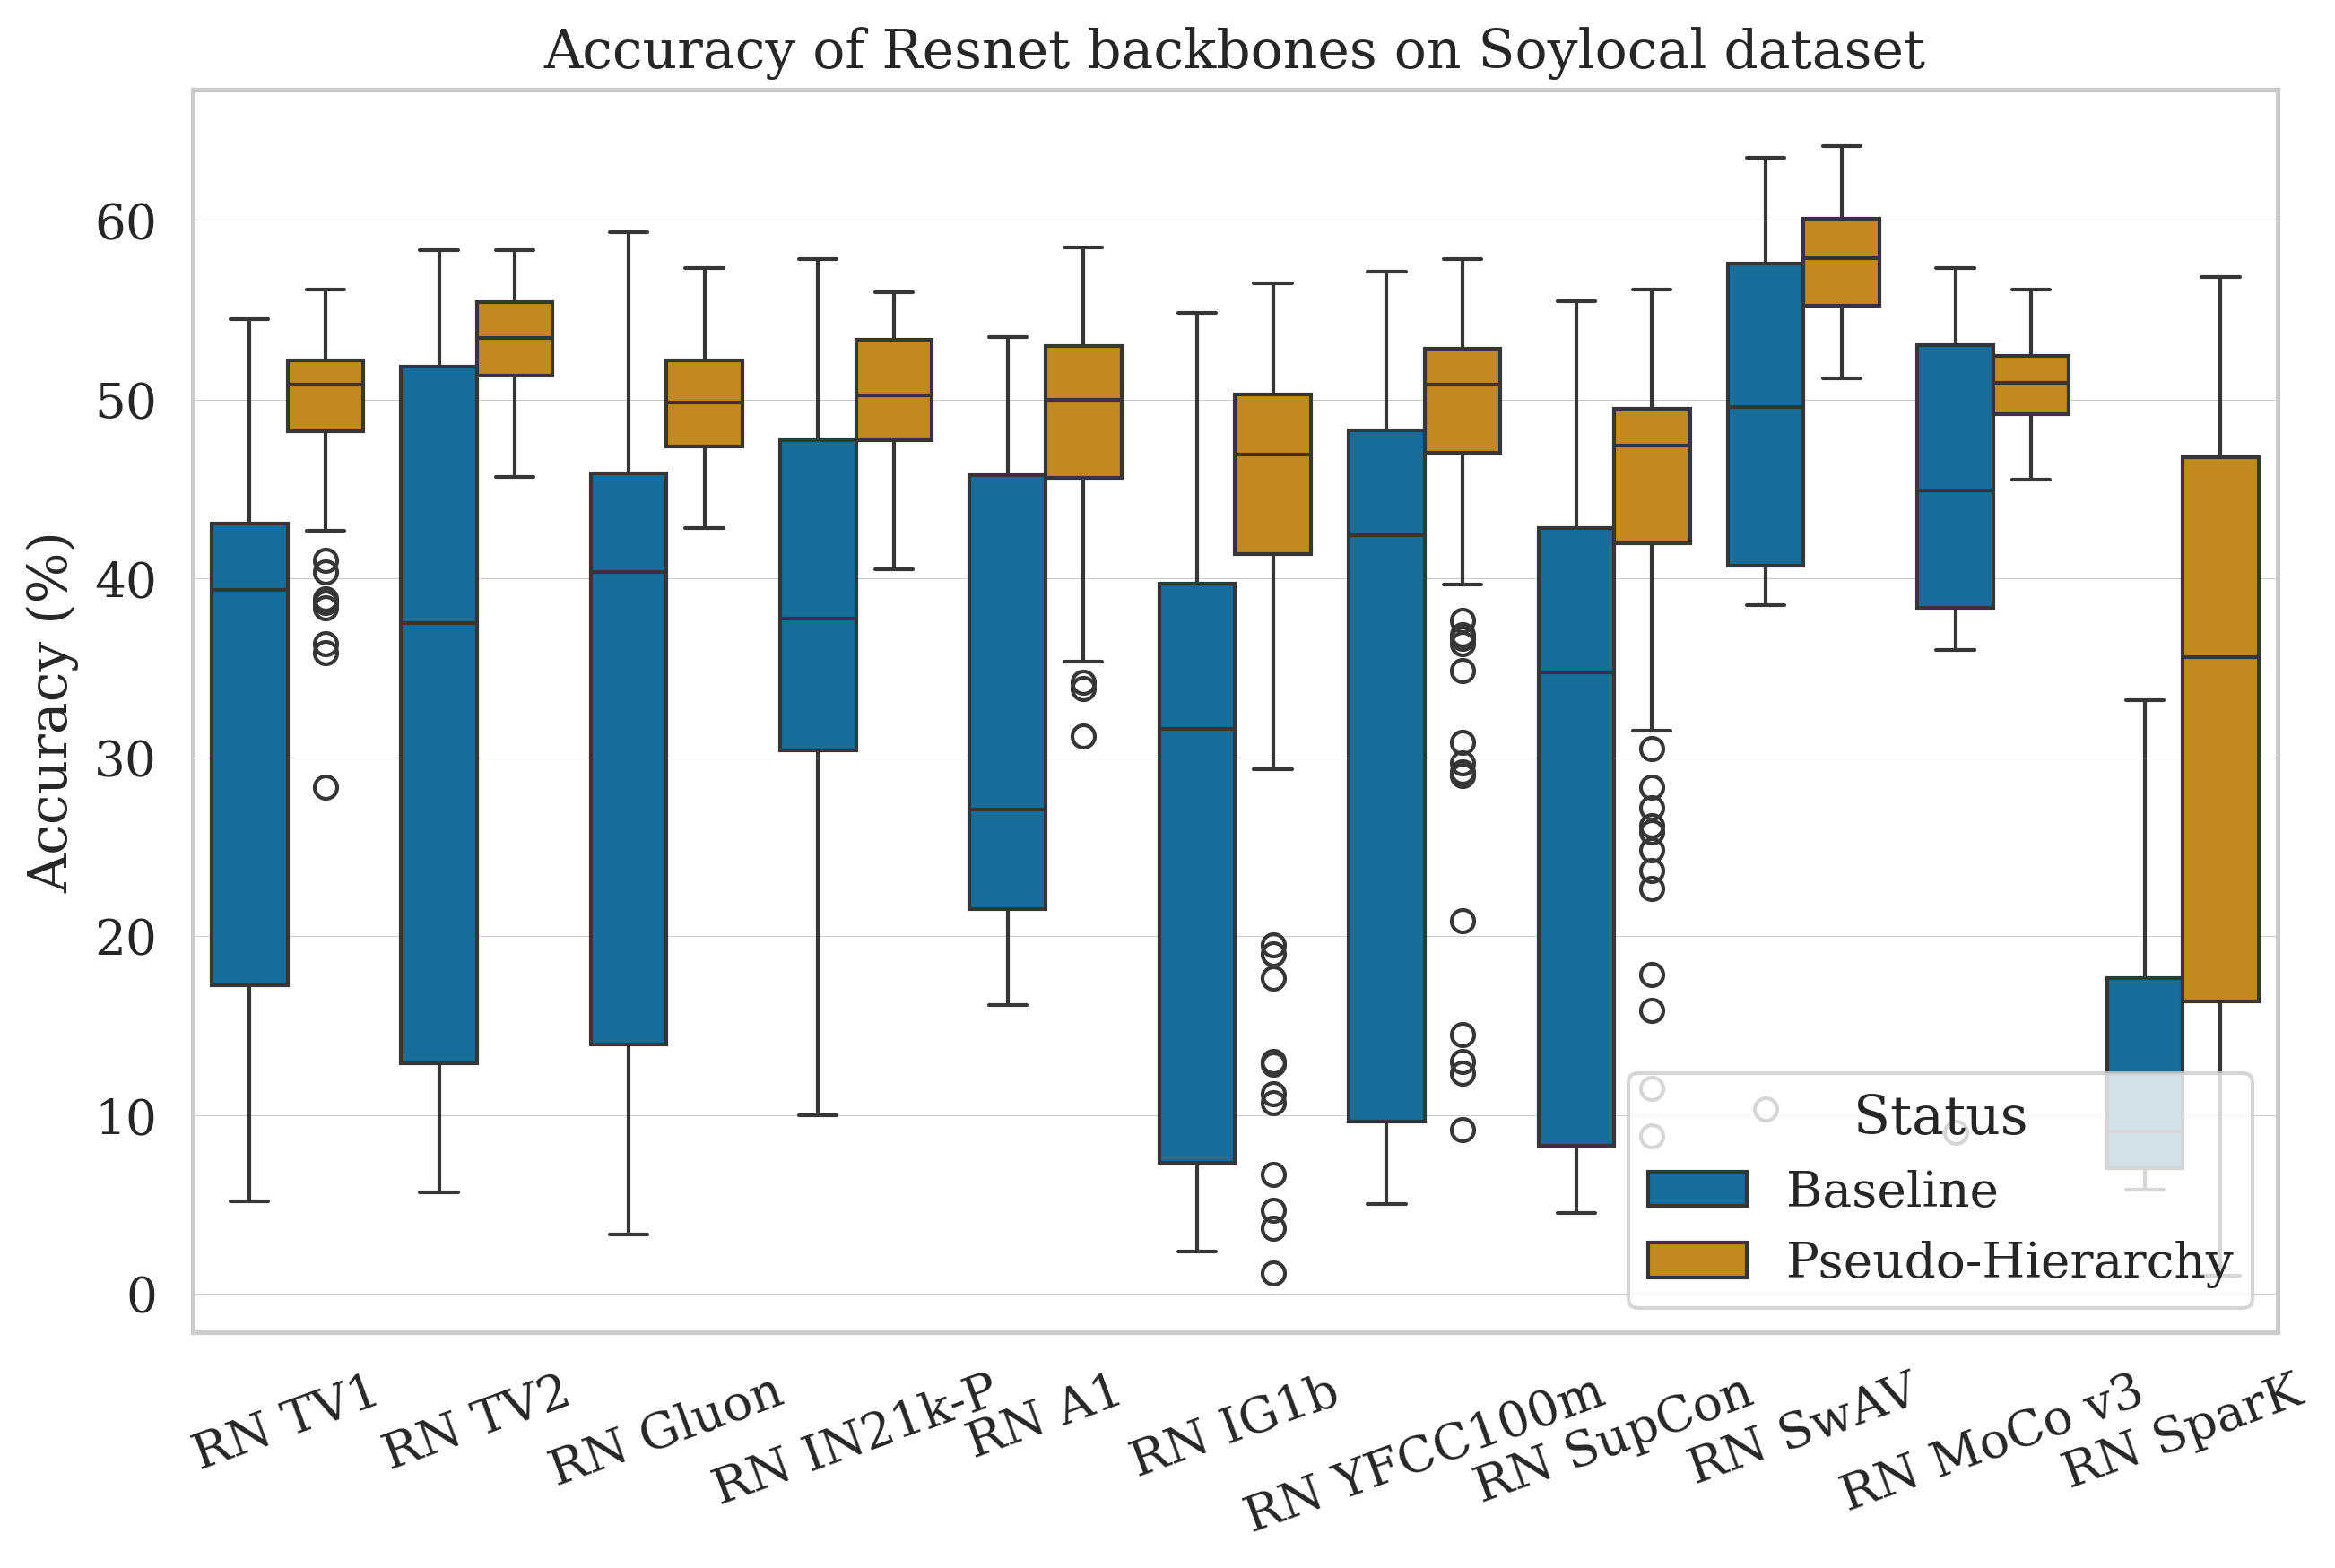
\includegraphics[width=\linewidth]{figures/compare_resnet_soylocal.png}
        \label{fig:resnet_soylocal}
    \end{minipage}
    \hspace{0.01\linewidth} % Reduce spacing
    \begin{minipage}{0.48\linewidth}
        \centering
        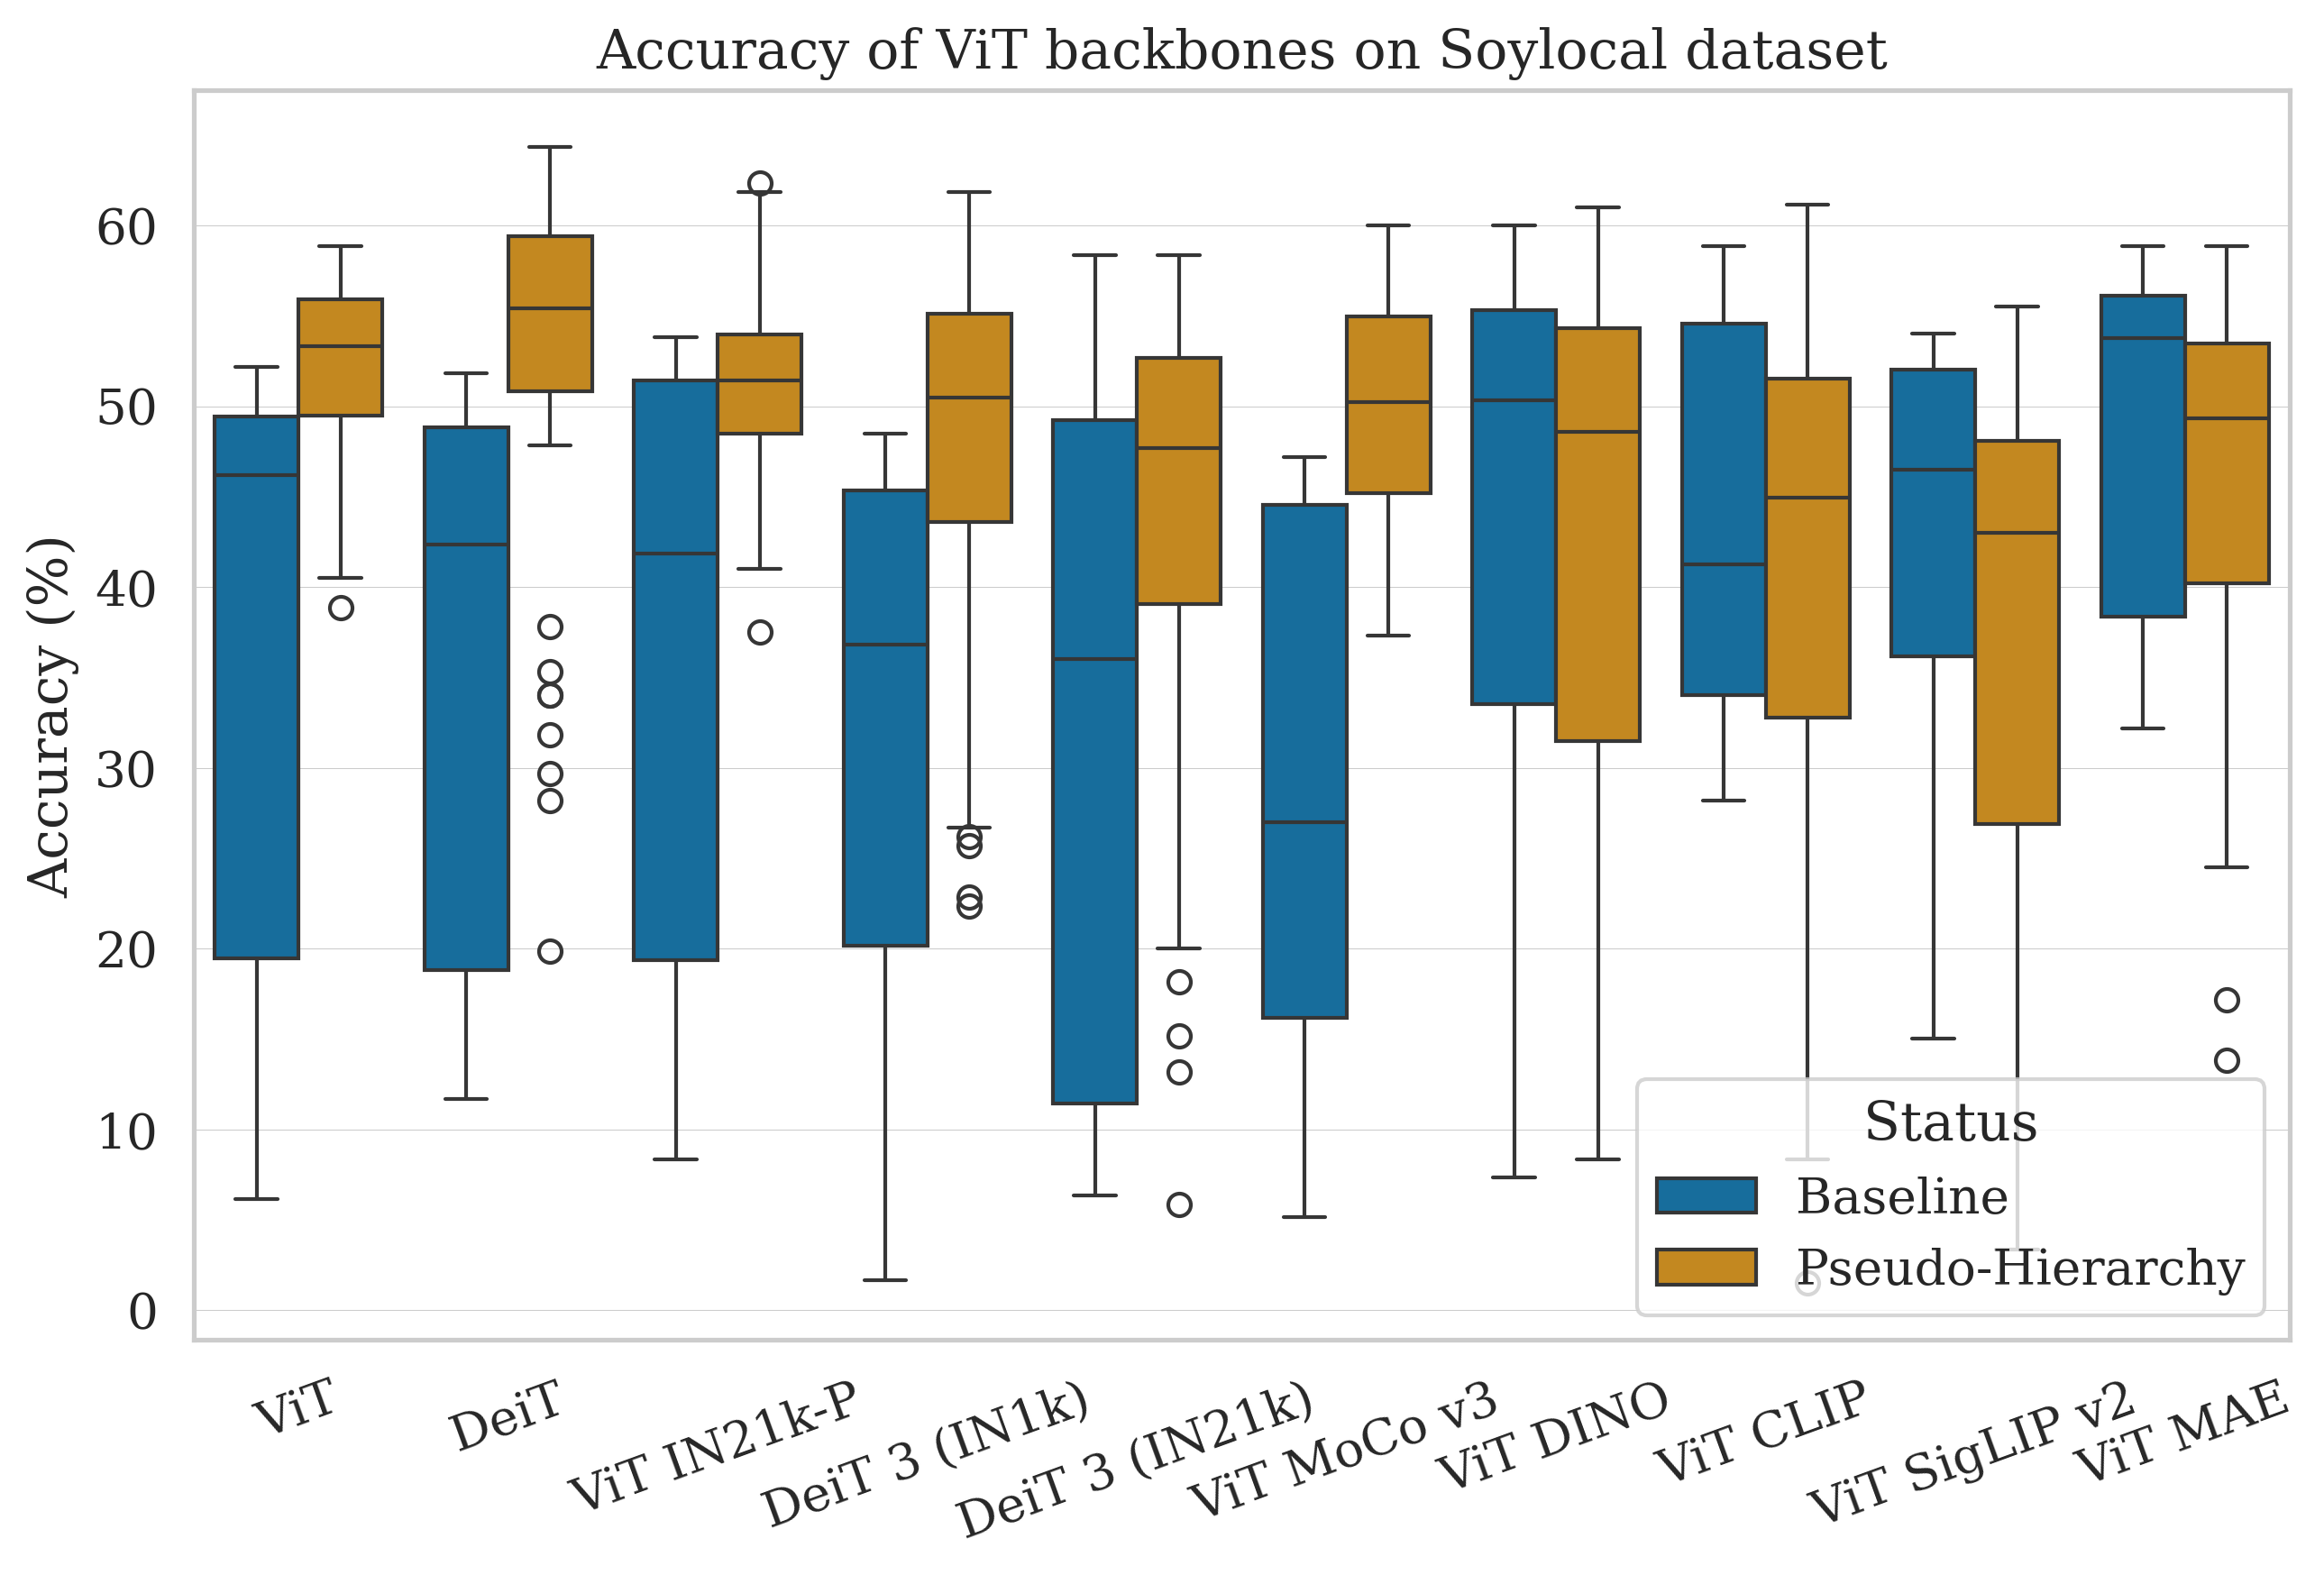
\includegraphics[width=\linewidth]{figures/compare_vit_soylocal.png}
        \label{fig:vit_soylocal}
    \end{minipage}
    \vspace{-0.55cm}
    \caption{Accuracy of 21 pretrained backbones on the Soylocal dataset under 7 different cluster ratios. Backbones are grouped by architecture, comparing ResNet variants (left) and ViT variants (right).}
    \label{fig_soylocal_models}
\end{figure*}

\section{Results}
\label{sec_results}
\subsection{Pseudo-Hierarchy Improves UFGIR Performance}
Figure~\ref{fig_pseudo_soylocal} compares the performance of 21 pretrained backbones on the SoyLocal dataset under different cluster ratios. Across all cluster ratios, incorporating HPH consistently outperforms the non-hierarchical baseline, showing that pseudo-hierarchies can effectively improve accuracy even on datasets without predefined hierarchical labels. Compared with non-hierarchical baseline, HPH achieves an absolute accuracy improvement of \textbf{up to 22.3\%}.

We observe that higher cluster ratios generally yield stronger performance. In particular, the 70\% and 90\% cluster ratios consistently rank among the best-performing ratios across the backbones. This indicates that preserving a larger number of pseudo-coarse categories better captures the semantic relationships between fine-grained classes.

\subsection{Performance Across Backbone Architectures}
Figure~\ref{fig_soylocal_models} compares the performance of HPH across 21 pretrained backbones, grouped into ResNet-based and Vision Transformer (ViT)-based architectures. In general, transformer-based backbones achieve higher classification accuracy than their CNN counterparts on the SoyLocal dataset, with models surpassing 60\% accuracy, whereas only ResNet SwAV reaches the same level among the ResNet models.

Despite the performance differences between architectures, HPH consistently improves the maximum accuracy of CNN and transformer backbones. Among the ResNet models, ResNet SparK achieves the largest improvement, increasing the maximum accuracy by \textbf{22.3\%} over the non-hierarchical baseline. For transformer models, DeiT obtains the largest gain of \textbf{12.5\%} to max accuracy over the non-hierarchical baseline.

In particular, DeiT model achieves the highest overall performance among all evaluated backbones, reaching a maximum accuracy of \textbf{64.3\%} with HPH. As DeiT is one of the most widely adopted standard Vision Transformer architectures, these results demonstrate that pseudo-hierarchical supervision can significantly improve the performance of commonly used model in FGIR tasks.

\begin{table}[!t]
\centering
\caption{Top-1 accuracies (\%) for SotA methods across 3 UFGIR benchmarks.}
\begin{tabular}{lccc}
\toprule
Method & Cotton & SoyAgeing-R1 & SoyLocal \\
\midrule
\textit{ViT-B models} \\
TransFG\cite{he_transfg_2022}   & 54.6 & 74.9 & 40.7 \\
SIM-Tr\cite{sun_sim-trans_2022}    & 54.6 & 69.9 & 25.0 \\
CSDNet\cite{fang_learning_2024}    & 57.9 & 75.2 & 46.2 \\
HPH (Ours) & \underline{68.3} & \underline{86.3} & \underline{58.7} \\
\midrule
\textit{DeiT-B models} \\
HPH (Ours)     & \textbf{72.5} & \textbf{89.6} & \textbf{64.3} \\
\bottomrule
\label{tab_compare_othersoy}
\end{tabular}
\end{table}

\subsection{Pseudo-Hierarchies on Low-Resource UFGIR Datasets}
To investigate the effectiveness of HPH in low-resource UFGIR, we extend our experiments to 2 additional datasets from the benchmark of Yu et al. \cite{yu_benchmark_2021}: Cotton and the SoyAgeing-R1 subset. Based on the results on SoyLocal, we evaluate only the 70\% and 90\% cluster ratios, which consistently achieved the strongest performance. We further select DeiT and the original ViT as representative backbones, as DeiT achieved the best performance on SoyLocal while both models are widely adopted standard Vision Transformer architectures.

In particular, all three datasets represent extremely low-resource UFGIR scenarios. SoyLocal contains 200 classes with 600 training images, Cotton contains 80 classes with 240 training images, and SoyAgeing-R1 contains 198 classes with 990 training images, corresponding to only 3, 3, and 5 training images per class, respectively. This limited supervision makes learning discriminative features particularly challenging.

Table~\ref{tab_compare_othersoy} summarizes the best performance obtained on the three datasets. HPH consistently outperforms all SotA baselines, with DeiT+HPH achieving the highest accuracy on every dataset. Compared to the strongest baseline, ViT+CSDNet, DeiT+HPH improves accuracy by 18.16\% on SoyLocal, 14.60\% on Cotton, and 14.45\% on SoyAgeing-R1. Although the magnitude of improvement varies across datasets, these consistent gains demonstrate that the effectiveness of HPH extends beyond a single benchmark and generalizes across SotA comparison methods.

From this perspective, the effectiveness of HPH can be attributed to the additional structure introduced through pseudo-hierarchies. By grouping fine-grained classes into macro pseudo-categories, HPH induces a curriculum learning process that gradually transitions from coarse to fine discrimination. This provides a more stable optimization path under limited data, leading to improved classification performance through curriculum learning.

\section{Conclusion}
\label{sec_conclusion}

We presented Hungarian Pseudo-Hierarchy (HPH), a framework that forms macro-categories by grouping semantically related fine-grained classes using bipartite matching. HPH enables curriculum learning within existing hierarchical frameworks, requiring no manually annotated taxonomies and thus generalizing readily to specialized domains where such hierarchies are unavailable. Across 21 pretrained CNN and Vision Transformer backbones, HPH consistently improves classification accuracy, with the best-performing DeiT backbone achieving \textbf{64.3\%} accuracy and an absolute improvement of \textbf{12.5\%} over the non-hierarchical baseline. Furthermore, HPH shows consistent benefits on low-resource UFGIR datasets containing only \textbf{3-5 training images per class}, improving accuracy over the ViT+CSDNet SoTA by \textbf{14.60\%} on Cotton, \textbf{14.45\%} on SoyAgeing-R1, and \textbf{18.16\%} on SoyLocal. These results show that automatically generated pseudo-hierarchies provide an effective and scalable alternative to manually annotated taxonomies, particularly for low-resource fine-grained recognition where curriculum learning offers the greatest benefit.

\bibliographystyle{IEEEtran}
\bibliography{sample-base}

\end{document}
